\documentclass[twoside]{book}

% Packages required by doxygen
\usepackage{fixltx2e}
\usepackage{calc}
\usepackage{doxygen}
\usepackage[export]{adjustbox} % also loads graphicx
\usepackage{graphicx}
\usepackage[utf8]{inputenc}
\usepackage{makeidx}
\usepackage{multicol}
\usepackage{multirow}
\PassOptionsToPackage{warn}{textcomp}
\usepackage{textcomp}
\usepackage[nointegrals]{wasysym}
\usepackage[table]{xcolor}

% Font selection
\usepackage[T1]{fontenc}
\usepackage[scaled=.90]{helvet}
\usepackage{courier}
\usepackage{amssymb}
\usepackage{sectsty}
\renewcommand{\familydefault}{\sfdefault}
\allsectionsfont{%
  \fontseries{bc}\selectfont%
  \color{darkgray}%
}
\renewcommand{\DoxyLabelFont}{%
  \fontseries{bc}\selectfont%
  \color{darkgray}%
}
\newcommand{\+}{\discretionary{\mbox{\scriptsize$\hookleftarrow$}}{}{}}

% Page & text layout
\usepackage{geometry}
\geometry{%
  a4paper,%
  top=2.5cm,%
  bottom=2.5cm,%
  left=2.5cm,%
  right=2.5cm%
}
\tolerance=750
\hfuzz=15pt
\hbadness=750
\setlength{\emergencystretch}{15pt}
\setlength{\parindent}{0cm}
\setlength{\parskip}{3ex plus 2ex minus 2ex}
\makeatletter
\renewcommand{\paragraph}{%
  \@startsection{paragraph}{4}{0ex}{-1.0ex}{1.0ex}{%
    \normalfont\normalsize\bfseries\SS@parafont%
  }%
}
\renewcommand{\subparagraph}{%
  \@startsection{subparagraph}{5}{0ex}{-1.0ex}{1.0ex}{%
    \normalfont\normalsize\bfseries\SS@subparafont%
  }%
}
\makeatother

% Headers & footers
\usepackage{fancyhdr}
\pagestyle{fancyplain}
\fancyhead[LE]{\fancyplain{}{\bfseries\thepage}}
\fancyhead[CE]{\fancyplain{}{}}
\fancyhead[RE]{\fancyplain{}{\bfseries\leftmark}}
\fancyhead[LO]{\fancyplain{}{\bfseries\rightmark}}
\fancyhead[CO]{\fancyplain{}{}}
\fancyhead[RO]{\fancyplain{}{\bfseries\thepage}}
\fancyfoot[LE]{\fancyplain{}{}}
\fancyfoot[CE]{\fancyplain{}{}}
\fancyfoot[RE]{\fancyplain{}{\bfseries\scriptsize Generated by Doxygen }}
\fancyfoot[LO]{\fancyplain{}{\bfseries\scriptsize Generated by Doxygen }}
\fancyfoot[CO]{\fancyplain{}{}}
\fancyfoot[RO]{\fancyplain{}{}}
\renewcommand{\footrulewidth}{0.4pt}
\renewcommand{\chaptermark}[1]{%
  \markboth{#1}{}%
}
\renewcommand{\sectionmark}[1]{%
  \markright{\thesection\ #1}%
}

% Indices & bibliography
\usepackage{natbib}
\usepackage[titles]{tocloft}
\setcounter{tocdepth}{3}
\setcounter{secnumdepth}{5}
\makeindex

% Hyperlinks (required, but should be loaded last)
\usepackage{ifpdf}
\ifpdf
  \usepackage[pdftex,pagebackref=true]{hyperref}
\else
  \usepackage[ps2pdf,pagebackref=true]{hyperref}
\fi
\hypersetup{%
  colorlinks=true,%
  linkcolor=blue,%
  citecolor=blue,%
  unicode%
}

% Custom commands
\newcommand{\clearemptydoublepage}{%
  \newpage{\pagestyle{empty}\cleardoublepage}%
}

\usepackage{caption}
\captionsetup{labelsep=space,justification=centering,font={bf},singlelinecheck=off,skip=4pt,position=top}

%===== C O N T E N T S =====

\begin{document}

% Titlepage & ToC
\hypersetup{pageanchor=false,
             bookmarksnumbered=true,
             pdfencoding=unicode
            }
\pagenumbering{alph}
\begin{titlepage}
\vspace*{7cm}
\begin{center}%
{\Large Graph\+Mongo \\[1ex]\large 1.\+0.\+0 }\\
\vspace*{1cm}
{\large Generated by Doxygen 1.8.12}\\
\end{center}
\end{titlepage}
\clearemptydoublepage
\pagenumbering{roman}
\tableofcontents
\clearemptydoublepage
\pagenumbering{arabic}
\hypersetup{pageanchor=true}

%--- Begin generated contents ---
\chapter{Namespace Index}
\section{Namespace List}
Here is a list of all documented namespaces with brief descriptions\+:\begin{DoxyCompactList}
\item\contentsline{section}{\hyperlink{namespacegraphmongo}{graphmongo} }{\pageref{namespacegraphmongo}}{}
\end{DoxyCompactList}

\chapter{Hierarchical Index}
\section{Class Hierarchy}
This inheritance list is sorted roughly, but not completely, alphabetically\+:\begin{DoxyCompactList}
\item set\begin{DoxyCompactList}
\item \contentsline{section}{graphmongo.\+Graph\+Mongo}{\pageref{classgraphmongo_1_1GraphMongo}}{}
\end{DoxyCompactList}
\item \contentsline{section}{graphmongo.\+Utils}{\pageref{classgraphmongo_1_1Utils}}{}
\item Mongo\+Client\begin{DoxyCompactList}
\item \contentsline{section}{graphmongo.\+Graph\+Mongo}{\pageref{classgraphmongo_1_1GraphMongo}}{}
\end{DoxyCompactList}
\end{DoxyCompactList}

\chapter{Class Index}
\section{Class List}
Here are the classes, structs, unions and interfaces with brief descriptions\+:\begin{DoxyCompactList}
\item\contentsline{section}{\hyperlink{classgraphmongo_1_1GraphMongo}{graphmongo.\+Graph\+Mongo} }{\pageref{classgraphmongo_1_1GraphMongo}}{}
\item\contentsline{section}{\hyperlink{classgraphmongo_1_1Utils}{graphmongo.\+Utils} }{\pageref{classgraphmongo_1_1Utils}}{}
\end{DoxyCompactList}

\chapter{Namespace Documentation}
\hypertarget{namespacegraphmongo}{}\section{graphmongo Namespace Reference}
\label{namespacegraphmongo}\index{graphmongo@{graphmongo}}
\subsection*{Classes}
\begin{DoxyCompactItemize}
\item 
class \hyperlink{classgraphmongo_1_1GraphMongo}{Graph\+Mongo}
\item 
class \hyperlink{classgraphmongo_1_1Utils}{Utils}
\end{DoxyCompactItemize}
\subsection*{Functions}
\begin{DoxyCompactItemize}
\item 
\hypertarget{namespacegraphmongo_a08837102d173acb3c80042dc53517e65}{}\label{namespacegraphmongo_a08837102d173acb3c80042dc53517e65} 
def {\bfseries Create\+Directed\+Graph} ()
\item 
\hypertarget{namespacegraphmongo_a39d1a2193f488c1724349e94c03f3aa1}{}\label{namespacegraphmongo_a39d1a2193f488c1724349e94c03f3aa1} 
def {\bfseries Create\+Simple\+Graph} ()
\item 
\hypertarget{namespacegraphmongo_a06974d1b9d1cf06218a4c34f94673e35}{}\label{namespacegraphmongo_a06974d1b9d1cf06218a4c34f94673e35} 
def {\bfseries Queries} ()
\item 
\hypertarget{namespacegraphmongo_aa9d9dfae9ff7c04f02610f4877f82c69}{}\label{namespacegraphmongo_aa9d9dfae9ff7c04f02610f4877f82c69} 
def {\bfseries Metrics} ()
\end{DoxyCompactItemize}
\subsection*{Variables}
\begin{DoxyCompactItemize}
\item 
\hypertarget{namespacegraphmongo_ab24c01e2ec223f8eff12287ef0940395}{}\label{namespacegraphmongo_ab24c01e2ec223f8eff12287ef0940395} 
{\bfseries parser} = argparse.\+Argument\+Parser(description=\char`\"{}Testing \hyperlink{classgraphmongo_1_1GraphMongo}{Graph\+Mongo} A\+PI\char`\"{})
\item 
\hypertarget{namespacegraphmongo_a697548046ee5b3292f3a1d4a64bdaa45}{}\label{namespacegraphmongo_a697548046ee5b3292f3a1d4a64bdaa45} 
{\bfseries required}
\item 
\hypertarget{namespacegraphmongo_a064485cb9d93569d342f20d33dd3ad52}{}\label{namespacegraphmongo_a064485cb9d93569d342f20d33dd3ad52} 
{\bfseries False}
\item 
\hypertarget{namespacegraphmongo_a9c92856e72bedfc8679568f66da1a335}{}\label{namespacegraphmongo_a9c92856e72bedfc8679568f66da1a335} 
{\bfseries help}
\item 
\hypertarget{namespacegraphmongo_a876a0120dd69b70c209a34661ea63ae4}{}\label{namespacegraphmongo_a876a0120dd69b70c209a34661ea63ae4} 
{\bfseries args} = parser.\+parse\+\_\+args()
\item 
\hypertarget{namespacegraphmongo_aac9de70b22072a15d613fb102198ac39}{}\label{namespacegraphmongo_aac9de70b22072a15d613fb102198ac39} 
{\bfseries graph} = \hyperlink{classgraphmongo_1_1GraphMongo}{Graph\+Mongo}(address=\textquotesingle{}localhost\textquotesingle{}, port=27018)
\item 
\hypertarget{namespacegraphmongo_a6ff4e4c73d73e9a679c164b7acb3cb97}{}\label{namespacegraphmongo_a6ff4e4c73d73e9a679c164b7acb3cb97} 
{\bfseries elems} = graph.\+Get\+Nodes().Get\+Neighbours().Fetch()
\end{DoxyCompactItemize}


\subsection{Detailed Description}
\begin{DoxyVerb}Copyright 2016, Oriol Mazariegos Canellas <oriol.mazariegos@gmail.com> 
 
This file is part of the GraphMongo framework.

GraphMongo is free software: you can redistribute it and/or modify
it under the terms of the GNU General Public License as published by
the Free Software Foundation, either version 3 of the License, or
(at your option) any later version.

GraphMongo is distributed in the hope that it will be useful,
but WITHOUT ANY WARRANTY; without even the implied warranty of
MERCHANTABILITY or FITNESS FOR A PARTICULAR PURPOSE.  See the
GNU General Public License for more details.

You should have received a copy of the GNU General Public License
along with GraphMongo.  If not, see <http://www.gnu.org/licenses/>.
\end{DoxyVerb}
 
\chapter{Class Documentation}
\hypertarget{classgraphmongo_1_1GraphMongo}{}\section{graphmongo.\+Graph\+Mongo Class Reference}
\label{classgraphmongo_1_1GraphMongo}\index{graphmongo.\+Graph\+Mongo@{graphmongo.\+Graph\+Mongo}}
Inheritance diagram for graphmongo.\+Graph\+Mongo\+:\begin{figure}[H]
\begin{center}
\leavevmode
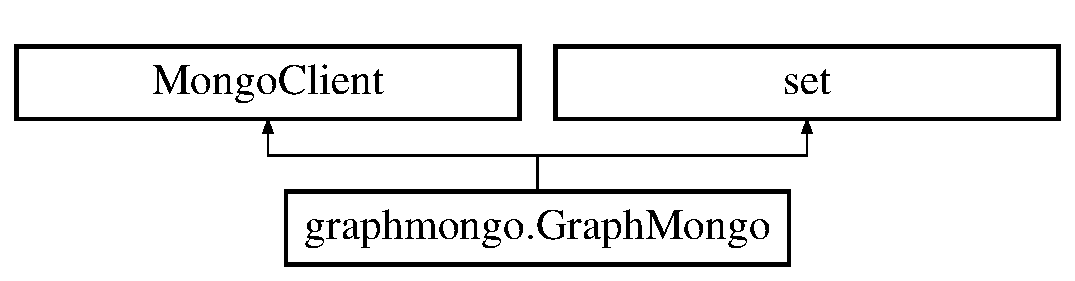
\includegraphics[height=2.000000cm]{classgraphmongo_1_1GraphMongo}
\end{center}
\end{figure}
\subsection*{Public Member Functions}
\begin{DoxyCompactItemize}
\item 
def \hyperlink{classgraphmongo_1_1GraphMongo_aab68747470d18460a87e296ff6e2a651}{\+\_\+\+\_\+init\+\_\+\+\_\+} (self, address=\char`\"{}localhost\char`\"{}, port=27017, dbname=\char`\"{}graph\char`\"{}, results=set(\mbox{[}$\,$\mbox{]}), connection=True)
\item 
def \hyperlink{classgraphmongo_1_1GraphMongo_a87d7b0d238de463bfffcae1a4ed7683f}{Clear\+Graph} (self, nodes=True, edges=True)
\item 
def \hyperlink{classgraphmongo_1_1GraphMongo_aa05e3a72c1e916e2d462c53e5f9a0bda}{Add\+Node} (self, node=None, label=None, weight=None, data=None)
\item 
def \hyperlink{classgraphmongo_1_1GraphMongo_add06fd535fdfe5dce31d0da7c06676fc}{Add\+Edge} (self, edge=None, label=None, weight=None, head=None, tail=None, data=None, type=\char`\"{}directed\char`\"{})
\item 
def \hyperlink{classgraphmongo_1_1GraphMongo_a09a2ea8847630acec5cdaab591ce82c0}{Update\+Node} (self, node=None)
\item 
def \hyperlink{classgraphmongo_1_1GraphMongo_a316443d72fac9aac57b3b3e74be96960}{Update\+Edge} (self, edge=None)
\item 
def \hyperlink{classgraphmongo_1_1GraphMongo_a3461c57941092ca2f34b253896594fc1}{Remove\+Node} (self, node=None)
\item 
def \hyperlink{classgraphmongo_1_1GraphMongo_a20e7f0726ec6951a51f9565702bd96e0}{Remove\+Edge} (self, edge=None)
\item 
def \hyperlink{classgraphmongo_1_1GraphMongo_a4ead15bb7429e6261ba3ff04d8e0ad34}{Get\+Edges} (self, edges=None, head=None, tail=None, label=None, weight=None, direction=None, query=None)
\item 
def \hyperlink{classgraphmongo_1_1GraphMongo_a08cfc20b885f77e0e22f9a9a7482dac6}{Get\+Nodes} (self, label=None, weight=None, direction=None, query=None)
\item 
def \hyperlink{classgraphmongo_1_1GraphMongo_ab820ea7237fd30bb51621800150e67d4}{Get\+Neighbours} (self, nodes=None, edges=None, label=None, weight=None, direction=None, query=None, disjunction=None)
\item 
def \hyperlink{classgraphmongo_1_1GraphMongo_af69f7a68ca1699c1586c71763c065d7c}{Vertex\+Count} (self)
\begin{DoxyCompactList}\small\item\em M\+E\+A\+S\+U\+R\+ES A\+ND M\+E\+T\+R\+I\+CS \#\#\#\#\#\#. \end{DoxyCompactList}\item 
def \hyperlink{classgraphmongo_1_1GraphMongo_a9c655ca4e219d5578b20f2e232212f1b}{Edge\+Count} (self)
\item 
def \hyperlink{classgraphmongo_1_1GraphMongo_a81f03a7b13d6f27cb959efcd9e16e7eb}{Vertex\+Degree} (self, nodes=None)
\item 
def \hyperlink{classgraphmongo_1_1GraphMongo_a05898a487478cb7409a2a510e5c716eb}{Graph\+Distance} (self, sources, targets=None, algorithm=None)
\begin{DoxyCompactList}\small\item\em D\+I\+S\+T\+A\+N\+C\+ES A\+L\+G\+O\+R\+I\+T\+H\+MS \#\#\#\#\#. \end{DoxyCompactList}\item 
def \hyperlink{classgraphmongo_1_1GraphMongo_a83f03c06d846ba61ba414a501825cdba}{Breadth\+First\+Search} (self, source, targets=None)
\item 
def \hyperlink{classgraphmongo_1_1GraphMongo_ad12c35ce9e8081ae46d42a7d19a8c8f8}{Dijkstra} (self, source, targets=None)
\end{DoxyCompactItemize}
\subsection*{Public Attributes}
\begin{DoxyCompactItemize}
\item 
\hypertarget{classgraphmongo_1_1GraphMongo_ab7afa11fffe20b5644ea8864fae5a37f}{}\label{classgraphmongo_1_1GraphMongo_ab7afa11fffe20b5644ea8864fae5a37f} 
{\bfseries address}
\item 
\hypertarget{classgraphmongo_1_1GraphMongo_aeab6f8f3e663cd0b7914c701be39821d}{}\label{classgraphmongo_1_1GraphMongo_aeab6f8f3e663cd0b7914c701be39821d} 
{\bfseries port}
\end{DoxyCompactItemize}
\subsection*{Static Public Attributes}
\begin{DoxyCompactItemize}
\item 
\hypertarget{classgraphmongo_1_1GraphMongo_a3465b2ec004b4beeafd681500e284bbe}{}\label{classgraphmongo_1_1GraphMongo_a3465b2ec004b4beeafd681500e284bbe} 
string {\bfseries address} = \char`\"{}localhost\char`\"{}
\item 
\hypertarget{classgraphmongo_1_1GraphMongo_a969049a5659c1599596cc6f5f7c2a94c}{}\label{classgraphmongo_1_1GraphMongo_a969049a5659c1599596cc6f5f7c2a94c} 
int {\bfseries port} = 27017
\end{DoxyCompactItemize}


\subsection{Detailed Description}
\begin{DoxyVerb}Graph class for mongodb database
\end{DoxyVerb}
 

\subsection{Constructor \& Destructor Documentation}
\hypertarget{classgraphmongo_1_1GraphMongo_aab68747470d18460a87e296ff6e2a651}{}\label{classgraphmongo_1_1GraphMongo_aab68747470d18460a87e296ff6e2a651} 
\index{graphmongo\+::\+Graph\+Mongo@{graphmongo\+::\+Graph\+Mongo}!\+\_\+\+\_\+init\+\_\+\+\_\+@{\+\_\+\+\_\+init\+\_\+\+\_\+}}
\index{\+\_\+\+\_\+init\+\_\+\+\_\+@{\+\_\+\+\_\+init\+\_\+\+\_\+}!graphmongo\+::\+Graph\+Mongo@{graphmongo\+::\+Graph\+Mongo}}
\subsubsection{\texorpdfstring{\+\_\+\+\_\+init\+\_\+\+\_\+()}{\_\_init\_\_()}}
{\footnotesize\ttfamily def graphmongo.\+Graph\+Mongo.\+\_\+\+\_\+init\+\_\+\+\_\+ (\begin{DoxyParamCaption}\item[{}]{self,  }\item[{}]{address = {\ttfamily \char`\"{}localhost\char`\"{}},  }\item[{}]{port = {\ttfamily 27017},  }\item[{}]{dbname = {\ttfamily \char`\"{}graph\char`\"{}},  }\item[{}]{results = {\ttfamily set(\mbox{[}\mbox{]})},  }\item[{}]{connection = {\ttfamily True} }\end{DoxyParamCaption})}

\begin{DoxyVerb}    @brief: init a connection with mongo ddbb
    @param address: ip address where the database is located 
    @param port: port where the database is listening
@param dbname: name for the graph database
@param results: list of ObjectId to initialize the instance with previous queries 
\end{DoxyVerb}
 

\subsection{Member Function Documentation}
\hypertarget{classgraphmongo_1_1GraphMongo_add06fd535fdfe5dce31d0da7c06676fc}{}\label{classgraphmongo_1_1GraphMongo_add06fd535fdfe5dce31d0da7c06676fc} 
\index{graphmongo\+::\+Graph\+Mongo@{graphmongo\+::\+Graph\+Mongo}!Add\+Edge@{Add\+Edge}}
\index{Add\+Edge@{Add\+Edge}!graphmongo\+::\+Graph\+Mongo@{graphmongo\+::\+Graph\+Mongo}}
\subsubsection{\texorpdfstring{Add\+Edge()}{AddEdge()}}
{\footnotesize\ttfamily def graphmongo.\+Graph\+Mongo.\+Add\+Edge (\begin{DoxyParamCaption}\item[{}]{self,  }\item[{}]{edge = {\ttfamily None},  }\item[{}]{label = {\ttfamily None},  }\item[{}]{weight = {\ttfamily None},  }\item[{}]{head = {\ttfamily None},  }\item[{}]{tail = {\ttfamily None},  }\item[{}]{data = {\ttfamily None},  }\item[{}]{type = {\ttfamily \char`\"{}directed\char`\"{}} }\end{DoxyParamCaption})}

\begin{DoxyVerb}@brief: create a new edge in the ddbb
@param edge: dictionary with an edge definition, params: _id, label, head (node 1), tail(node 2) and data
@param label: relation name of the edge
@param weight: weight of the edge
@param data: extra information
@param type: type of the edge, "directed" or "simple"
@return: edge created in the ddbb, otherwise an error is returned as dictionary with status ko\end{DoxyVerb}
 \hypertarget{classgraphmongo_1_1GraphMongo_aa05e3a72c1e916e2d462c53e5f9a0bda}{}\label{classgraphmongo_1_1GraphMongo_aa05e3a72c1e916e2d462c53e5f9a0bda} 
\index{graphmongo\+::\+Graph\+Mongo@{graphmongo\+::\+Graph\+Mongo}!Add\+Node@{Add\+Node}}
\index{Add\+Node@{Add\+Node}!graphmongo\+::\+Graph\+Mongo@{graphmongo\+::\+Graph\+Mongo}}
\subsubsection{\texorpdfstring{Add\+Node()}{AddNode()}}
{\footnotesize\ttfamily def graphmongo.\+Graph\+Mongo.\+Add\+Node (\begin{DoxyParamCaption}\item[{}]{self,  }\item[{}]{node = {\ttfamily None},  }\item[{}]{label = {\ttfamily None},  }\item[{}]{weight = {\ttfamily None},  }\item[{}]{data = {\ttfamily None} }\end{DoxyParamCaption})}

\begin{DoxyVerb}@brief: create a new node in the ddbb
@param node: dictionary with a node definition, params: _id, label and data
@param label: type name of the node
@param weight: weight of the node
@param data: extra information
@return: node created in the ddbb otherwise an error is returned as dictionary with status=ko  
\end{DoxyVerb}
 \hypertarget{classgraphmongo_1_1GraphMongo_a83f03c06d846ba61ba414a501825cdba}{}\label{classgraphmongo_1_1GraphMongo_a83f03c06d846ba61ba414a501825cdba} 
\index{graphmongo\+::\+Graph\+Mongo@{graphmongo\+::\+Graph\+Mongo}!Breadth\+First\+Search@{Breadth\+First\+Search}}
\index{Breadth\+First\+Search@{Breadth\+First\+Search}!graphmongo\+::\+Graph\+Mongo@{graphmongo\+::\+Graph\+Mongo}}
\subsubsection{\texorpdfstring{Breadth\+First\+Search()}{BreadthFirstSearch()}}
{\footnotesize\ttfamily def graphmongo.\+Graph\+Mongo.\+Breadth\+First\+Search (\begin{DoxyParamCaption}\item[{}]{self,  }\item[{}]{source,  }\item[{}]{targets = {\ttfamily None} }\end{DoxyParamCaption})}

\begin{DoxyVerb}@brief: gives the distance and previous node from source vertex to target vertex for unweighted graphs. complexity=O(|E|+|V|)
@param source: ObjectId of source node
@param target: list of ObjectId of target nodes
@return: dictionary with relation of source and targets. fist the tag "distance" give the distance from source to target and in the "from" the node where we have arrived to the current node
\end{DoxyVerb}
 \hypertarget{classgraphmongo_1_1GraphMongo_a87d7b0d238de463bfffcae1a4ed7683f}{}\label{classgraphmongo_1_1GraphMongo_a87d7b0d238de463bfffcae1a4ed7683f} 
\index{graphmongo\+::\+Graph\+Mongo@{graphmongo\+::\+Graph\+Mongo}!Clear\+Graph@{Clear\+Graph}}
\index{Clear\+Graph@{Clear\+Graph}!graphmongo\+::\+Graph\+Mongo@{graphmongo\+::\+Graph\+Mongo}}
\subsubsection{\texorpdfstring{Clear\+Graph()}{ClearGraph()}}
{\footnotesize\ttfamily def graphmongo.\+Graph\+Mongo.\+Clear\+Graph (\begin{DoxyParamCaption}\item[{}]{self,  }\item[{}]{nodes = {\ttfamily True},  }\item[{}]{edges = {\ttfamily True} }\end{DoxyParamCaption})}

\begin{DoxyVerb}@brief: remove all nodes and edges of the ddbb taking account the params
@param nodes: option to delete all nodes
@param edges: option to delete all edges
\end{DoxyVerb}
 \hypertarget{classgraphmongo_1_1GraphMongo_ad12c35ce9e8081ae46d42a7d19a8c8f8}{}\label{classgraphmongo_1_1GraphMongo_ad12c35ce9e8081ae46d42a7d19a8c8f8} 
\index{graphmongo\+::\+Graph\+Mongo@{graphmongo\+::\+Graph\+Mongo}!Dijkstra@{Dijkstra}}
\index{Dijkstra@{Dijkstra}!graphmongo\+::\+Graph\+Mongo@{graphmongo\+::\+Graph\+Mongo}}
\subsubsection{\texorpdfstring{Dijkstra()}{Dijkstra()}}
{\footnotesize\ttfamily def graphmongo.\+Graph\+Mongo.\+Dijkstra (\begin{DoxyParamCaption}\item[{}]{self,  }\item[{}]{source,  }\item[{}]{targets = {\ttfamily None} }\end{DoxyParamCaption})}

\begin{DoxyVerb}@brief: gives the distance and previous node from source vertex to target vertex for weighted graph. complexity=O((|E|+|V|) log |V|) = O(|E| log |V|) because we are using priority queue
@param source: ObjectId of source node
@param target: list of ObjectId of target nodes
@return: dictionary with relation of source and targets. fist the tag "distance" give the distance from source to target and in the "from" the node where we have arrived to the current node
\end{DoxyVerb}
 \hypertarget{classgraphmongo_1_1GraphMongo_a9c655ca4e219d5578b20f2e232212f1b}{}\label{classgraphmongo_1_1GraphMongo_a9c655ca4e219d5578b20f2e232212f1b} 
\index{graphmongo\+::\+Graph\+Mongo@{graphmongo\+::\+Graph\+Mongo}!Edge\+Count@{Edge\+Count}}
\index{Edge\+Count@{Edge\+Count}!graphmongo\+::\+Graph\+Mongo@{graphmongo\+::\+Graph\+Mongo}}
\subsubsection{\texorpdfstring{Edge\+Count()}{EdgeCount()}}
{\footnotesize\ttfamily def graphmongo.\+Graph\+Mongo.\+Edge\+Count (\begin{DoxyParamCaption}\item[{}]{self }\end{DoxyParamCaption})}

\begin{DoxyVerb}@brief: gives a count of the number of edges in the graph
@return: numeber of edges
\end{DoxyVerb}
 \hypertarget{classgraphmongo_1_1GraphMongo_a4ead15bb7429e6261ba3ff04d8e0ad34}{}\label{classgraphmongo_1_1GraphMongo_a4ead15bb7429e6261ba3ff04d8e0ad34} 
\index{graphmongo\+::\+Graph\+Mongo@{graphmongo\+::\+Graph\+Mongo}!Get\+Edges@{Get\+Edges}}
\index{Get\+Edges@{Get\+Edges}!graphmongo\+::\+Graph\+Mongo@{graphmongo\+::\+Graph\+Mongo}}
\subsubsection{\texorpdfstring{Get\+Edges()}{GetEdges()}}
{\footnotesize\ttfamily def graphmongo.\+Graph\+Mongo.\+Get\+Edges (\begin{DoxyParamCaption}\item[{}]{self,  }\item[{}]{edges = {\ttfamily None},  }\item[{}]{head = {\ttfamily None},  }\item[{}]{tail = {\ttfamily None},  }\item[{}]{label = {\ttfamily None},  }\item[{}]{weight = {\ttfamily None},  }\item[{}]{direction = {\ttfamily None},  }\item[{}]{query = {\ttfamily None} }\end{DoxyParamCaption})}

\begin{DoxyVerb}@brief: get list of edges given id's, label or quering
@param edges: list of edges
@param label: label of the node or relation
@param weight: weight of the node or relation
@param direction: direction of the relation, "head|tail"
@param query: mongodb expression query applyed in the ddbb
@return list of edges, otherwise an error is returned as dictionary with status ko
\end{DoxyVerb}
 \hypertarget{classgraphmongo_1_1GraphMongo_ab820ea7237fd30bb51621800150e67d4}{}\label{classgraphmongo_1_1GraphMongo_ab820ea7237fd30bb51621800150e67d4} 
\index{graphmongo\+::\+Graph\+Mongo@{graphmongo\+::\+Graph\+Mongo}!Get\+Neighbours@{Get\+Neighbours}}
\index{Get\+Neighbours@{Get\+Neighbours}!graphmongo\+::\+Graph\+Mongo@{graphmongo\+::\+Graph\+Mongo}}
\subsubsection{\texorpdfstring{Get\+Neighbours()}{GetNeighbours()}}
{\footnotesize\ttfamily def graphmongo.\+Graph\+Mongo.\+Get\+Neighbours (\begin{DoxyParamCaption}\item[{}]{self,  }\item[{}]{nodes = {\ttfamily None},  }\item[{}]{edges = {\ttfamily None},  }\item[{}]{label = {\ttfamily None},  }\item[{}]{weight = {\ttfamily None},  }\item[{}]{direction = {\ttfamily None},  }\item[{}]{query = {\ttfamily None},  }\item[{}]{disjunction = {\ttfamily None} }\end{DoxyParamCaption})}

\begin{DoxyVerb}@brief: get list of related nodes given nodes or related nodes with edges
@param nodes: list of ObjectId's of nodes
@param edges: list of ObjectId's of edges
@param label: label of the node or relation
@param weight: weight of the node or relation
@param direction: direction of the relation, "head|tail"
@param query: mongodb expression query applyed in the ddbb
        @param disjunction: option to delete in the result the previous queries
@return: graphmongo instance with list of nodes, otherwise an error is returned as dictionary with status ko
\end{DoxyVerb}
 \hypertarget{classgraphmongo_1_1GraphMongo_a08cfc20b885f77e0e22f9a9a7482dac6}{}\label{classgraphmongo_1_1GraphMongo_a08cfc20b885f77e0e22f9a9a7482dac6} 
\index{graphmongo\+::\+Graph\+Mongo@{graphmongo\+::\+Graph\+Mongo}!Get\+Nodes@{Get\+Nodes}}
\index{Get\+Nodes@{Get\+Nodes}!graphmongo\+::\+Graph\+Mongo@{graphmongo\+::\+Graph\+Mongo}}
\subsubsection{\texorpdfstring{Get\+Nodes()}{GetNodes()}}
{\footnotesize\ttfamily def graphmongo.\+Graph\+Mongo.\+Get\+Nodes (\begin{DoxyParamCaption}\item[{}]{self,  }\item[{}]{label = {\ttfamily None},  }\item[{}]{weight = {\ttfamily None},  }\item[{}]{direction = {\ttfamily None},  }\item[{}]{query = {\ttfamily None} }\end{DoxyParamCaption})}

\begin{DoxyVerb}    @brief: get list of nodes given label, weight or other kind of query
    @param label: label of the node or relation
    @param weight: weight of the node or relation
    @param query: mongodb expression query applyed in the ddbb
    @return: graphmongo instance with list of nodes, otherwise an error is returned as dictionary with status ko\end{DoxyVerb}
 \hypertarget{classgraphmongo_1_1GraphMongo_a05898a487478cb7409a2a510e5c716eb}{}\label{classgraphmongo_1_1GraphMongo_a05898a487478cb7409a2a510e5c716eb} 
\index{graphmongo\+::\+Graph\+Mongo@{graphmongo\+::\+Graph\+Mongo}!Graph\+Distance@{Graph\+Distance}}
\index{Graph\+Distance@{Graph\+Distance}!graphmongo\+::\+Graph\+Mongo@{graphmongo\+::\+Graph\+Mongo}}
\subsubsection{\texorpdfstring{Graph\+Distance()}{GraphDistance()}}
{\footnotesize\ttfamily def graphmongo.\+Graph\+Mongo.\+Graph\+Distance (\begin{DoxyParamCaption}\item[{}]{self,  }\item[{}]{sources,  }\item[{}]{targets = {\ttfamily None},  }\item[{}]{algorithm = {\ttfamily None} }\end{DoxyParamCaption})}



D\+I\+S\+T\+A\+N\+C\+ES A\+L\+G\+O\+R\+I\+T\+H\+MS \#\#\#\#\#. 

\begin{DoxyVerb}@brief: gives the distance from source vertes to target vertex
@param sources: list of ObjectId's of source nodes
@param targets: list of ObjectId's of target nodes      
@param algorithm: function to be called as a parameter. the function have to follow the input/output like __GraphDistance(self, source, target=None) generic function
@return: dictionary with relation of sources and targets. This relation is a list of intermediate ObjectId nodes and weights
\end{DoxyVerb}
 \hypertarget{classgraphmongo_1_1GraphMongo_a20e7f0726ec6951a51f9565702bd96e0}{}\label{classgraphmongo_1_1GraphMongo_a20e7f0726ec6951a51f9565702bd96e0} 
\index{graphmongo\+::\+Graph\+Mongo@{graphmongo\+::\+Graph\+Mongo}!Remove\+Edge@{Remove\+Edge}}
\index{Remove\+Edge@{Remove\+Edge}!graphmongo\+::\+Graph\+Mongo@{graphmongo\+::\+Graph\+Mongo}}
\subsubsection{\texorpdfstring{Remove\+Edge()}{RemoveEdge()}}
{\footnotesize\ttfamily def graphmongo.\+Graph\+Mongo.\+Remove\+Edge (\begin{DoxyParamCaption}\item[{}]{self,  }\item[{}]{edge = {\ttfamily None} }\end{DoxyParamCaption})}

\begin{DoxyVerb}@brief: remove an specific edge head the ddbb
@param edge: dictionary with an edge definition, params: _id, label, head (node 1), tail(node 2) and data
@return: dictionary with status 'ok' or 'ko'
\end{DoxyVerb}
 \hypertarget{classgraphmongo_1_1GraphMongo_a3461c57941092ca2f34b253896594fc1}{}\label{classgraphmongo_1_1GraphMongo_a3461c57941092ca2f34b253896594fc1} 
\index{graphmongo\+::\+Graph\+Mongo@{graphmongo\+::\+Graph\+Mongo}!Remove\+Node@{Remove\+Node}}
\index{Remove\+Node@{Remove\+Node}!graphmongo\+::\+Graph\+Mongo@{graphmongo\+::\+Graph\+Mongo}}
\subsubsection{\texorpdfstring{Remove\+Node()}{RemoveNode()}}
{\footnotesize\ttfamily def graphmongo.\+Graph\+Mongo.\+Remove\+Node (\begin{DoxyParamCaption}\item[{}]{self,  }\item[{}]{node = {\ttfamily None} }\end{DoxyParamCaption})}

\begin{DoxyVerb}@brief: remove an specific node from the ddbb
@param node: dictionary with a node definition, params: _id, label and data
@return: dictionary with status 'ok' or 'ko' 
\end{DoxyVerb}
 \hypertarget{classgraphmongo_1_1GraphMongo_a316443d72fac9aac57b3b3e74be96960}{}\label{classgraphmongo_1_1GraphMongo_a316443d72fac9aac57b3b3e74be96960} 
\index{graphmongo\+::\+Graph\+Mongo@{graphmongo\+::\+Graph\+Mongo}!Update\+Edge@{Update\+Edge}}
\index{Update\+Edge@{Update\+Edge}!graphmongo\+::\+Graph\+Mongo@{graphmongo\+::\+Graph\+Mongo}}
\subsubsection{\texorpdfstring{Update\+Edge()}{UpdateEdge()}}
{\footnotesize\ttfamily def graphmongo.\+Graph\+Mongo.\+Update\+Edge (\begin{DoxyParamCaption}\item[{}]{self,  }\item[{}]{edge = {\ttfamily None} }\end{DoxyParamCaption})}

\begin{DoxyVerb}@brief: update desired edge, _id, head and tail cannot be updated, remove edge and create another one
@param edge: dictionary with an edge definition, params: _id, label, head (node 1), tail(node 2) and data
@return: edge updated in the ddbb otherwise an error is returned as dictionary with status=ko
\end{DoxyVerb}
 \hypertarget{classgraphmongo_1_1GraphMongo_a09a2ea8847630acec5cdaab591ce82c0}{}\label{classgraphmongo_1_1GraphMongo_a09a2ea8847630acec5cdaab591ce82c0} 
\index{graphmongo\+::\+Graph\+Mongo@{graphmongo\+::\+Graph\+Mongo}!Update\+Node@{Update\+Node}}
\index{Update\+Node@{Update\+Node}!graphmongo\+::\+Graph\+Mongo@{graphmongo\+::\+Graph\+Mongo}}
\subsubsection{\texorpdfstring{Update\+Node()}{UpdateNode()}}
{\footnotesize\ttfamily def graphmongo.\+Graph\+Mongo.\+Update\+Node (\begin{DoxyParamCaption}\item[{}]{self,  }\item[{}]{node = {\ttfamily None} }\end{DoxyParamCaption})}

\begin{DoxyVerb}@brief: update desired node, _id and label field cannot be updated, remove node and create another one
@param node: dictionary with a node definition, params: _id, label and data
@return: node updated in the ddbb otherwise an error is returned as dictionary with status=ko
\end{DoxyVerb}
 \hypertarget{classgraphmongo_1_1GraphMongo_af69f7a68ca1699c1586c71763c065d7c}{}\label{classgraphmongo_1_1GraphMongo_af69f7a68ca1699c1586c71763c065d7c} 
\index{graphmongo\+::\+Graph\+Mongo@{graphmongo\+::\+Graph\+Mongo}!Vertex\+Count@{Vertex\+Count}}
\index{Vertex\+Count@{Vertex\+Count}!graphmongo\+::\+Graph\+Mongo@{graphmongo\+::\+Graph\+Mongo}}
\subsubsection{\texorpdfstring{Vertex\+Count()}{VertexCount()}}
{\footnotesize\ttfamily def graphmongo.\+Graph\+Mongo.\+Vertex\+Count (\begin{DoxyParamCaption}\item[{}]{self }\end{DoxyParamCaption})}



M\+E\+A\+S\+U\+R\+ES A\+ND M\+E\+T\+R\+I\+CS \#\#\#\#\#\#. 

\begin{DoxyVerb}@brief: gives a count of the number of vertices in the graph
@return: number of nodes
\end{DoxyVerb}
 \hypertarget{classgraphmongo_1_1GraphMongo_a81f03a7b13d6f27cb959efcd9e16e7eb}{}\label{classgraphmongo_1_1GraphMongo_a81f03a7b13d6f27cb959efcd9e16e7eb} 
\index{graphmongo\+::\+Graph\+Mongo@{graphmongo\+::\+Graph\+Mongo}!Vertex\+Degree@{Vertex\+Degree}}
\index{Vertex\+Degree@{Vertex\+Degree}!graphmongo\+::\+Graph\+Mongo@{graphmongo\+::\+Graph\+Mongo}}
\subsubsection{\texorpdfstring{Vertex\+Degree()}{VertexDegree()}}
{\footnotesize\ttfamily def graphmongo.\+Graph\+Mongo.\+Vertex\+Degree (\begin{DoxyParamCaption}\item[{}]{self,  }\item[{}]{nodes = {\ttfamily None} }\end{DoxyParamCaption})}

\begin{DoxyVerb}@brief: gives the list of vertex degrees for all nodes or nodes passed in the parameter in the graph
@param nodes: list of nodes
@return: dictionary with the nodeid and its degree
\end{DoxyVerb}
 

The documentation for this class was generated from the following file\+:\begin{DoxyCompactItemize}
\item 
/home/mazas/api/graphmongo/graphmongo.\+py\end{DoxyCompactItemize}

\hypertarget{classgraphmongo_1_1Utils}{}\section{graphmongo.\+Utils Class Reference}
\label{classgraphmongo_1_1Utils}\index{graphmongo.\+Utils@{graphmongo.\+Utils}}
\subsection*{Public Member Functions}
\begin{DoxyCompactItemize}
\item 
def \hyperlink{classgraphmongo_1_1Utils_ac2f4fcdf9f82ea6f876e092d2a7375fc}{wrap\+Elems} (self, elem)
\end{DoxyCompactItemize}


\subsection{Detailed Description}
\begin{DoxyVerb}Utils class for check, validations and wrappers
\end{DoxyVerb}
 

\subsection{Member Function Documentation}
\hypertarget{classgraphmongo_1_1Utils_ac2f4fcdf9f82ea6f876e092d2a7375fc}{}\label{classgraphmongo_1_1Utils_ac2f4fcdf9f82ea6f876e092d2a7375fc} 
\index{graphmongo\+::\+Utils@{graphmongo\+::\+Utils}!wrap\+Elems@{wrap\+Elems}}
\index{wrap\+Elems@{wrap\+Elems}!graphmongo\+::\+Utils@{graphmongo\+::\+Utils}}
\subsubsection{\texorpdfstring{wrap\+Elems()}{wrapElems()}}
{\footnotesize\ttfamily def graphmongo.\+Utils.\+wrap\+Elems (\begin{DoxyParamCaption}\item[{}]{self,  }\item[{}]{elem }\end{DoxyParamCaption})}

\begin{DoxyVerb}@brief: change elem type to list of ObjectId's
@param elem: object with elements
@return: list of ObjectId's 
\end{DoxyVerb}
 

The documentation for this class was generated from the following file\+:\begin{DoxyCompactItemize}
\item 
/home/mazas/api/graphmongo/graphmongo.\+py\end{DoxyCompactItemize}

%--- End generated contents ---

% Index
\backmatter
\newpage
\phantomsection
\clearemptydoublepage
\addcontentsline{toc}{chapter}{Index}
\printindex

\end{document}
